\documentclass[10pt,twocolumn,a4paper]{article}

\usepackage[utf8]{inputenc}
\usepackage[T1]{fontenc}
\usepackage{lmodern}
\usepackage[a4paper,margin=1.5cm,columnsep=0.6cm]{geometry}
\usepackage{microtype}
\usepackage{amsmath}
\usepackage{graphicx}
\usepackage{xcolor}
\usepackage{booktabs}
\usepackage{enumitem}
\usepackage[font=small,labelfont=bf,skip=2pt]{caption}
\usepackage[numbers,sort&compress]{natbib}
\usepackage[colorlinks=true,linkcolor=black,citecolor=blue!50!black,urlcolor=blue!50!black]{hyperref}

\setlist{itemsep=1pt,topsep=2pt,parsep=0pt,leftmargin=1.3em}
\setlength{\parskip}{1.5pt}
\setlength{\textfloatsep}{6pt plus 2pt minus 2pt}
\setlength{\floatsep}{5pt plus 2pt minus 2pt}
\setlength{\dbltextfloatsep}{6pt plus 2pt minus 2pt}
\setlength{\abovedisplayskip}{3pt}\setlength{\belowdisplayskip}{3pt}
\makeatletter
\renewcommand\section{\@startsection{section}{1}{\z@}{-6pt plus -2pt}{3pt}{\normalfont\large\bfseries}}
\renewcommand\subsection{\@startsection{subsection}{2}{\z@}{-4pt plus -1pt}{2pt}{\normalfont\normalsize\bfseries}}
\makeatother
\bibliographystyle{unsrtnat}
\setlength{\bibsep}{1pt}
\graphicspath{{figures_run8/}}

\title{\vspace{-1.2cm}\textbf{Device-Related Thrombus after LAA Occlusion in Case~3:\\ Image Assessment and Haemodynamic Risk}}
\author{Hugo Jal\\[1pt]\small Modelling of Organs and Systems, Universitat Pompeu Fabra}
\date{\small 07/11/2026\vspace{-0.45cm}}

\begin{document}

\twocolumn[
\maketitle
\begin{abstract}
\noindent \textbf{Is there a device-related thrombus (DRT)?} I do not think so: on the CT the blood in front of the occluder enhances like the rest of the atrium, and the only dark spots, next to the metal hub, are darker than any clot could be (metal artefact). \textbf{Is the patient at risk of one?} Yes. A flow simulation of the left atrium (LA) shows almost still blood against the device while the mitral valve is closed, recirculation just in front of it, and the lowest, most oscillating wall shear of the atrium around it.
\end{abstract}
\vspace{2pt}
{\begin{center}
\begin{minipage}[b]{0.205\textwidth}\centering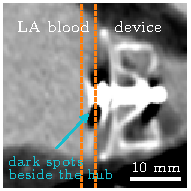
\includegraphics[width=\linewidth]{fig_ct_axis.pdf}\\[-1pt]\small (a)\end{minipage}\hfill
\begin{minipage}[b]{0.25\textwidth}\centering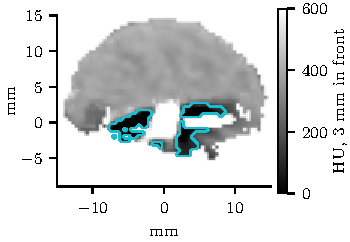
\includegraphics[width=\linewidth]{fig_ct_rays.pdf}\\[-1pt]\small (b)\end{minipage}\hfill
\begin{minipage}[b]{0.30\textwidth}\centering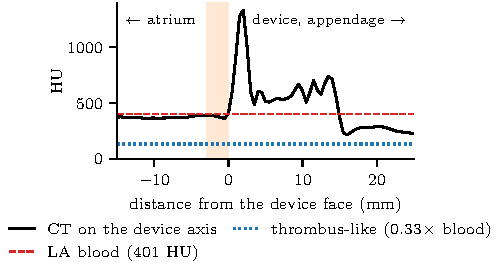
\includegraphics[width=\linewidth]{fig_ct_profile.pdf}\\[-1pt]\small (c)\end{minipage}\hfill
\begin{minipage}[b]{0.20\textwidth}\centering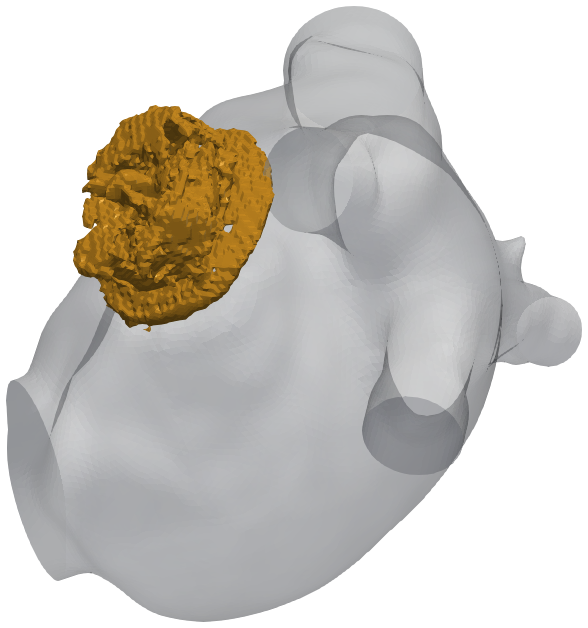
\includegraphics[width=\linewidth]{pv_anatomy_wire.png}\\[-1pt]\small (d)\end{minipage}
\captionof{figure}{Is there a thrombus on the device? (a) Plain CT through the device axis, atrium on the left; dashed: the 3\,mm in front of the device where a thrombus would be. (b) Mean attenuation in those 3\,mm seen from the atrium (cyan: below one third of the blood). (c) Attenuation along the device axis. (d) LA model and device wire frame.}
\label{fig:ct}
\end{center}}
\vspace{2pt}
]

\section{Introduction}
Left atrial appendage occlusion (LAAO) closes the appendage with a device to prevent strokes in patients with atrial fibrillation. A known complication is a device-related thrombus (DRT) on its atrial face: it is not frequent, but it clearly raises the risk of stroke \citep{Dukkipati2018}. Patient-specific flow simulations have linked DRT to slow blood and to low, oscillating wall shear stress around the device \citep{Zhong2024,Vogl2024}. For Case~3 I answer two questions: is there a DRT on the CT, and is the patient at risk of one?

\begin{figure*}[t]
\centering
\begin{minipage}[b]{0.19\textwidth}\centering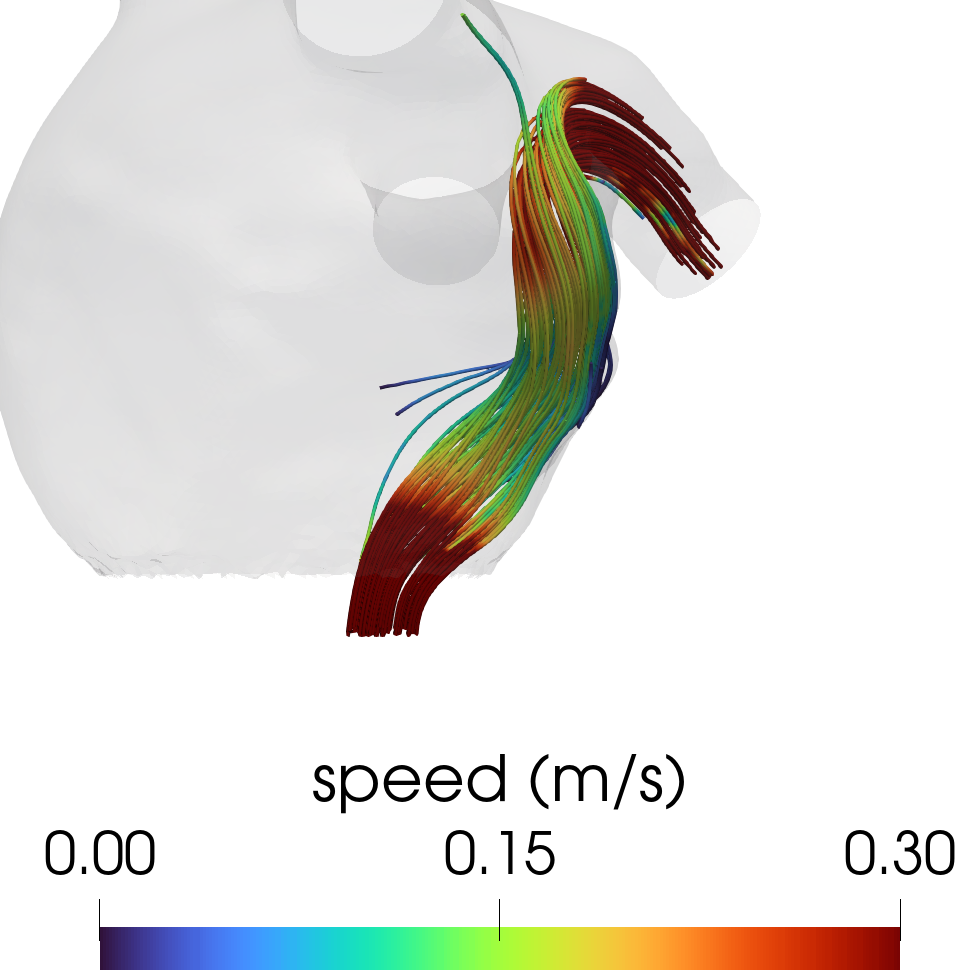
\includegraphics[width=\linewidth]{streamlines_side_filling_t306.png}\\[-1pt]\small (a) filling peak\end{minipage}\hfill
\begin{minipage}[b]{0.19\textwidth}\centering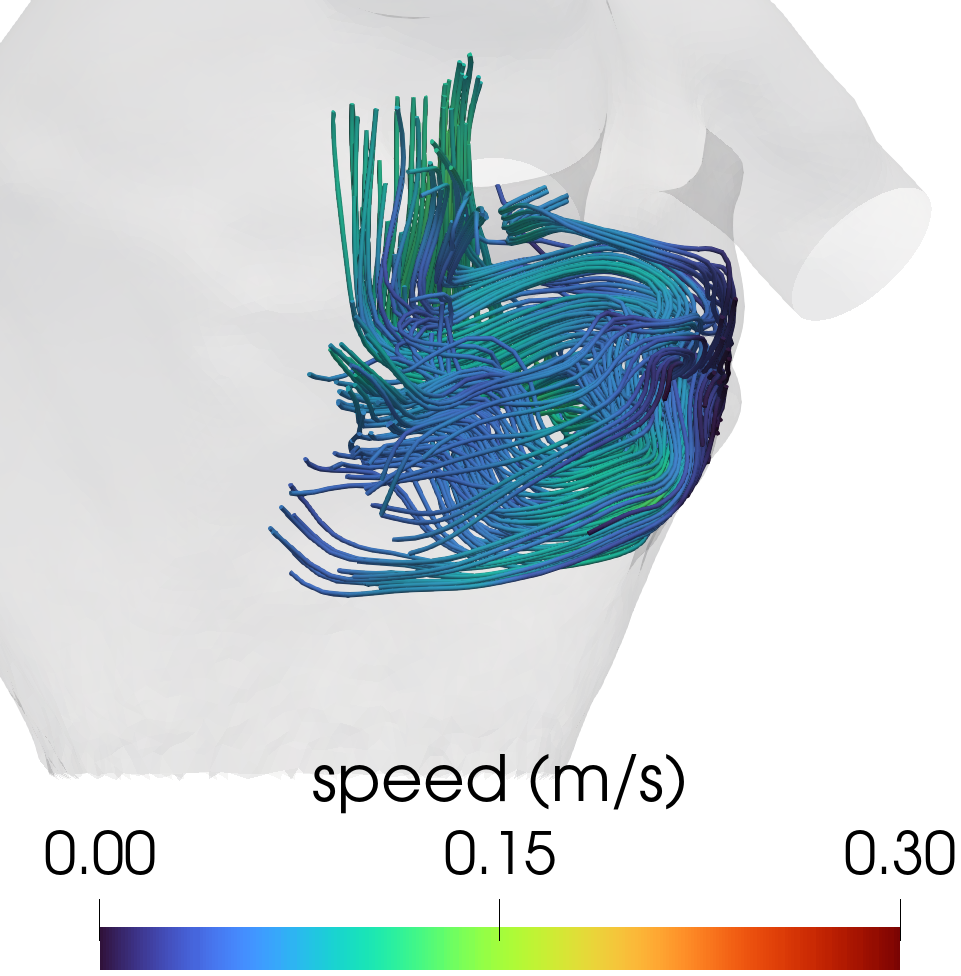
\includegraphics[width=\linewidth]{streamlines_side_systole_t290.png}\\[-1pt]\small (b) valve closed\end{minipage}\hfill
\begin{minipage}[b]{0.19\textwidth}\centering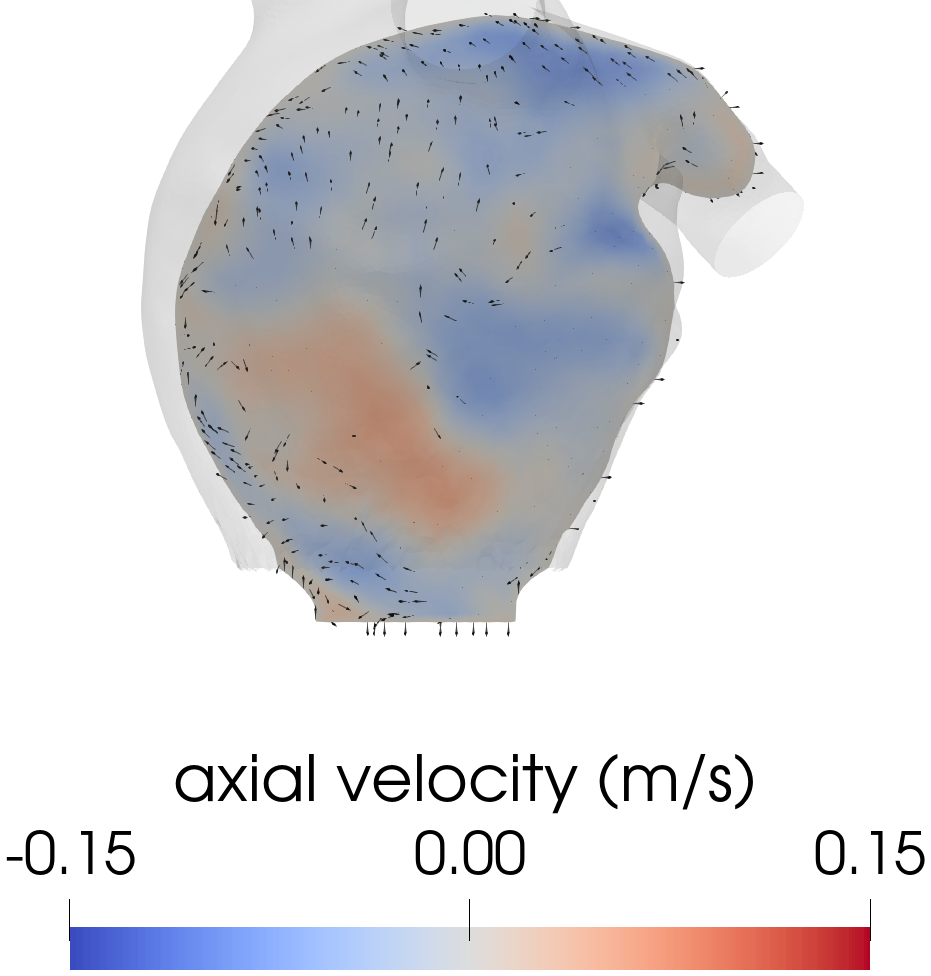
\includegraphics[width=\linewidth]{longaxis_slice_systole_t290.png}\\[-1pt]\small (c) valve closed\end{minipage}\hfill
\begin{minipage}[b]{0.19\textwidth}\centering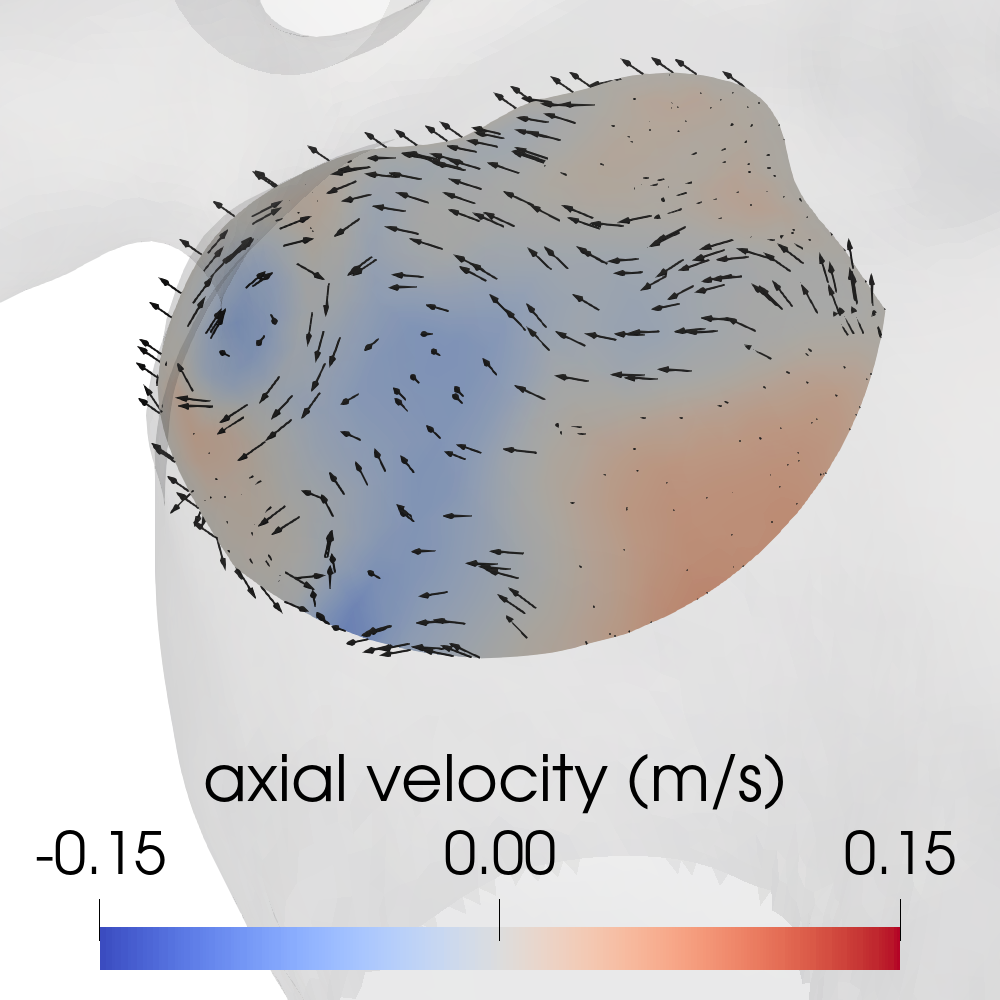
\includegraphics[width=\linewidth]{section_8mm_systole_t290.png}\\[-1pt]\small (d) valve closed, 8\,mm\end{minipage}\hfill
\begin{minipage}[b]{0.19\textwidth}\centering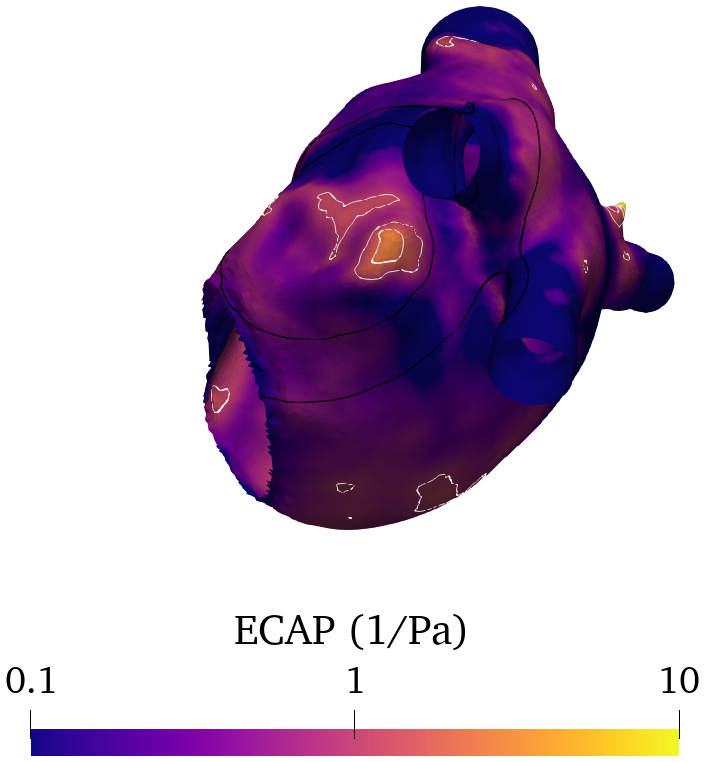
\includegraphics[width=\linewidth]{pv_wall_ecap_dev.png}\\[-1pt]\small (e) ECAP\end{minipage}
\caption{Flow and wall shear in front of the device (not drawn; on the right in a--c). (a, b) Streamlines started 5\,mm in front of the device. (c) Velocity along the device axis (red: towards the device) on a plane through it and (d) on the section 8\,mm in front, seen from the atrium. (e) ECAP over the beat; black lines: 10 and 20\,mm from the device.}
\label{fig:flow}
\end{figure*}

\section{Methods}
\subsection{Segmentation and mesh}
The contrast CT (diastolic phase) was segmented in 3D Slicer by manual thresholding of the blood, refined by painting and erasing within the threshold range. The four pulmonary veins (PVs) were kept up to their first branch and the device was left out of the blood volume. The device (Amulet-type, a disc and a lobe) was segmented manually, and its wire frame separately from a gamma-transformed CT ($\gamma=0.3$; Fig.~\ref{fig:ct}d). Each PV was cut perpendicular to its trunk and extended with a 10\,mm cylinder of the same area (diameters 9--18\,mm), and the mitral valve (MV) was cut on the annulus plane found in the CT, made the $z$ axis, and narrowed to a 5.3\,cm$^2$ orifice (normal: 4--6\,cm$^2$). The volume was meshed with 272\,000 tetrahedra in Gmsh.

\subsection{Looking for a thrombus on the CT}
On contrast CT a DRT is a dark (hypoattenuating) thickening on the atrial face of the device: clot does not take up contrast, so it is darker than the blood around it. A layer thicker than 3\,mm is considered a definite DRT \citep{Agudelo2021,Korsholm2019}. Since there is no single HU cut-off, I compared the blood just in front of the device with the blood of the whole atrium. Along lines parallel to the device axis, coming from the atrium, I averaged the attenuation over the last 3\,mm before the device and marked as suspicious anything below one third of the atrial blood, roughly the appendage-to-aorta ratio that separates thrombus from slow blood in \citep{Li2022}.

\subsection{Flow simulation and analysis}
The flow was solved in Ansys Fluent as transient and laminar, with Newtonian blood ($\rho=1060$\,kg/m$^3$, $\mu=3.5$\,mPa\,s). The PVs received the course pressure curve and the MV the course velocity curve (80\,mL per beat, 5.5\,L/min \citep{KawelBoehm2020}) together with its motion along the valve axis (up to 9\,mm), handled with a dynamic mesh. I simulated four heartbeats ($\Delta t=0.01$\,s) and analysed the last. Every time step reached the residual criteria (continuity $5\cdot10^{-3}$, velocity $10^{-3}$), and the last two beats differed by less than 1\,\% in mitral flow. From the wall shear stress $\boldsymbol\tau_w$ over the beat I computed TAWSS ($\tfrac1T\!\int|\boldsymbol\tau_w|dt$), OSI ($\tfrac12(1-|\!\int\boldsymbol\tau_w dt|/\!\int|\boldsymbol\tau_w|dt)$) and ECAP $=$ OSI/TAWSS, which is high where shear is low and changes direction \citep{Vogl2024}. On sections parallel to the device face, 2--16\,mm from it, I measured at every time step the share of slow blood ($|v|<0.05$\,m/s) and the shares flowing towards the device and back into the atrium. If both are large at once, the blood recirculates.

\begin{figure}[t]
\centering
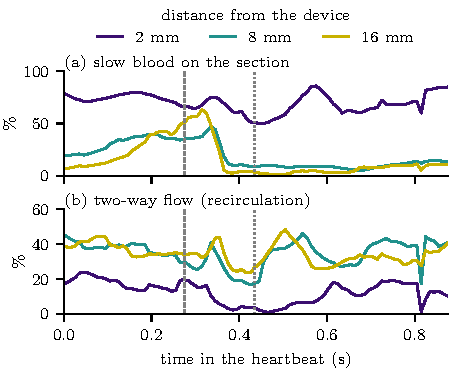
\includegraphics[width=0.9\columnwidth]{fig_sections.pdf}
\caption{Sections parallel to the device face at 2, 8 and 16\,mm. (a) Share of slow blood ($|v|<0.05$\,m/s). (b) Share of the section flowing the less common way (towards or away from the device); high values mean recirculation. Dashed: valve closed (Fig.~\ref{fig:flow}b--d); dotted: filling peak (Fig.~\ref{fig:flow}a).}
\label{fig:sections}
\end{figure}

\begin{figure}[t]
\centering
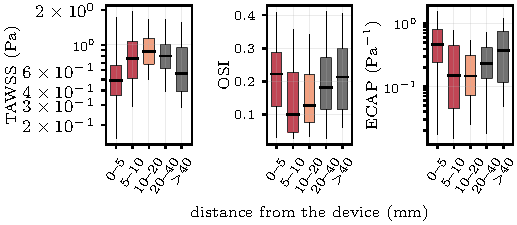
\includegraphics[width=0.9\columnwidth]{fig_bands.pdf}
\caption{TAWSS, OSI and ECAP of the wall grouped by distance from the device (box: interquartile range, line: median; red: near the device).}
\label{fig:wall}
\end{figure}

\section{Results}
\subsection{Is there a thrombus?}
My first look was the plane through the device axis (Fig.~\ref{fig:ct}a): the grey, contrast-filled blood reaches the device face along almost its whole height. However, right next to the bright hub there are two black spots, so I measured the whole disc. Over about 90\,\% of the face the 3\,mm of blood in front of the device has 375\,HU, practically the atrial blood (401\,HU; Fig.~\ref{fig:ct}b). The other 10\,\% (cyan) lies only on both sides of the hub, which saturates the scanner. Along the axis the attenuation stays at the blood level up to the device (Fig.~\ref{fig:ct}c). I do not think these spots are a thrombus: in 92\,\% of them the attenuation drops below 0\,HU (median minimum $-$414\,HU), which a clot, being soft tissue, cannot have, and dark bands on both sides of a dense metal part are the typical streak artefact. Even as tissue they would be under 3\,mm thick. I also noticed that the appendage behind the device still has about 280\,HU, above the 100\,HU used to call it sealed \citep{Agudelo2021}, so some contrast may pass the device.


\subsection{Flow near the device}
The flow is physiological (80\,mL per beat; fastest blood, about 1\,m/s, in the mitral orifice). At the peak of filling, the blood from the veins forms a fast stream that passes beside the device on its way to the valve without entering the space in front of it (Fig.~\ref{fig:flow}a). While the valve is closed the picture is different: the blood in front of the device is slow and swirls on itself (Fig.~\ref{fig:flow}b), with flow towards the device and back into the atrium side by side (Fig.~\ref{fig:flow}c), and an in-plane vortex on the 8\,mm section (Fig.~\ref{fig:flow}d).

The sections make this quantitative (Fig.~\ref{fig:sections}). At 2\,mm from the device, 70\,\% of the blood is slower than 0.05\,m/s on average, and it never drops below half, not even at the filling peak, when at 8 and 16\,mm the slow share falls to 10\,\% or less (Fig.~\ref{fig:sections}a). This layer is still, not recirculating (Fig.~\ref{fig:sections}b). Further out it is the opposite: at 5--16\,mm at least 20\,\% of each section flows each way during more than 90\,\% of the beat, most clearly just after the filling peak, so there the blood recirculates. The space in front of the device is a dead end: the main stream passes by, and blood that enters it turns around instead of leaving.


\subsection{Wall shear stress}
In the ECAP map (Fig.~\ref{fig:flow}e) I see high values around the entrance of the occluded appendage, inside the 10\,mm line, but the very highest values are in small separate patches on the roof and on the lower wall. So I grouped the wall by distance to the device (Fig.~\ref{fig:wall}): within 5\,mm the TAWSS is the lowest (30\,\% below the rest of the wall) and the OSI the highest of all groups, and the median ECAP is about 1.7 times that of the rest of the atrium. The wall within 10\,mm is only 10\,\% of the atrium but holds 38\,\% of the area with ECAP above 2\,Pa$^{-1}$.


\section{Discussion and conclusion}
Still blood on the device face, recirculation in front of it and low, oscillating shear around it are the conditions that patient-specific studies relate to DRT \citep{Zhong2024,Vogl2024}. Limitations: the artefact could hide a very small thrombus right on the hub; the boundary conditions are generic course curves and the device is not a solid in the flow, so I compared regions of the same atrium rather than using fixed thresholds.

\textbf{Conclusion.} I do not see a device-related thrombus in this CT, but \textbf{the patient is at risk of developing one}, because the blood in front of the device is the stillest of the atrium. Follow-up imaging is advisable.

\clearpage
\onecolumn
{\small\bibliography{references}}

\end{document}
